\documentclass[11pt]{article}

% basic packages
\usepackage[margin=1in]{geometry}
\usepackage[pdftex]{graphicx}
\usepackage{amsmath,amssymb,amsthm}
\usepackage{custom}
\usepackage{lipsum}

\usepackage{xcolor}
\usepackage{tikz-cd}

\usepackage[most]{tcolorbox}

% page formatting
\usepackage{fancyhdr}
\pagestyle{fancy}

\renewcommand{\sectionmark}[1]{\markright{\textsf{\arabic{section}. #1}}}
\renewcommand{\subsectionmark}[1]{}
\lhead{\textbf{\thepage} \ \ \nouppercase{\rightmark}}
\chead{}
\rhead{}
\lfoot{}
\cfoot{}
\rfoot{}
\setlength{\headheight}{14pt}

\linespread{1.03} % give a little extra room
\setlength{\parindent}{0.2in} % reduce paragraph indent a bit
\setcounter{secnumdepth}{2} % no numbered subsubsections
\setcounter{tocdepth}{2} % no subsubsections in ToC


%%%%%%%%%%%%%%%%%%%%%%%%%%%%%%%%%%%%%%%%%%%%%%%%%%%%%%%%%%%%%%%%%
% CUSTOM BOXES AND STUFF
\newtcolorbox{redbox}{colback=red!5!white,colframe=red!75!black, breakable}
\newtcolorbox{bluebox}{colback=blue!5!white,colframe=blue!75!black, breakable}
%%%%%%%%%%%%%%%%%%%%%%%%%%%%%%%%%%%%%%%%%%%%%%%%%%%%%%%%%%%%%%%%%


\begin{document}

% make title page
\thispagestyle{empty}
\bigskip \
\vspace{0.1cm}

\begin{center}
{\fontsize{22}{22} \selectfont Physics Directed Reading Program}
\vskip 16pt
{\fontsize{36}{36} \selectfont \bf \sffamily Topology and Geometry in Physics}
\vskip 24pt
{\fontsize{18}{18} \selectfont \rmfamily Keshav Balwant Deoskar} 
\vskip 6pt
{\fontsize{14}{14} \selectfont \ttfamily kdeoskar@berkeley.edu} 
\vskip 24pt
\end{center}

% {\parindent0pt \baselineskip=15.5pt \lipsum[1-4]} 

% make table of contents
% \newpage

These are some notes from the Phyiscs Directed Reading Program (PDRP) group headed by graduate student Vi Hong. Our group was interested in learning about topology and geometry with applications (primarily) to condensed matter physics.   
\\
\\
I'm writing these notes primarily to flesh out my own understanding, and so there's some content I've added which may not have actually been covered in the reading group. The order of topics is slightly different, and there may be some content missing.

\vskip 0.5cm
\begin{redbox}
    Please feel free to point out and errors / suggestions if you spot any via email! There's likely to be at least a few. 
\end{redbox}

% \microtoc
\tableofcontents 

% main 

%%%%%%%%%%%%%%%%%%%%%%%%%%%%%%%%%%%%%%%%%%%%%%
\newpage
\section{Quick Review of Topology}
%%%%%%%%%%%%%%%%%%%%%%%%%%%%%%%%%%%%%%%%%%%%%%
\vskip 0.5cm

\subsection{Open sets and Continuity}

\subsection{Topological Manifolds}

\subsection{Differentiable Structure}

\subsection{Tangent and Cotangent Spaces}

\subsection{Tangent and Cotangent Bundles}

%%%%%%%%%%%%%%%%%%%%%%%%%%%%%%%%%%%%%%%%%%%%%%
\newpage
\section{Bundles}
%%%%%%%%%%%%%%%%%%%%%%%%%%%%%%%%%%%%%%%%%%%%%%

\subsection{Vector Bundles}
This section follows \cite{LeeSM}.

\begin{definition}
    Let $M$ be a topological space. Then, given some other topological space $E$ and a \textit{surjective continuous map} $\pi \text{ : } E \rightarrow M$, the triple $(E, \pi, M)$ is called a \textit{(real) vector bundle of rank $k$ over $M$} if: 
    \begin{enumerate}[label=(\alph*)]
        \item For each $p \in M$, the fiber $E_p = \pi^{-1}(p)$ has $k-$dimensional vector space structure.
        \item For each $p \in M$, there exists some (open) neighborhood $ p \in U \subseteq M$ and homomorphism $\Phi \text{ : } \pi^{-1}(U) \rightarrow U \times \mathbb{R}^k$ such that 
        \begin{itemize}
            \item $\pi_U \circ \Phi = \pi$ ($\pi_U \text{ : } U \times \mathbb{R}^k \rightarrow U$ is the projection down to $U$)
            \item for every $q \in U$, $\restr{\Phi}{E_q} \text{ : } E_q \rightarrow \{q\} \times \mathbb{R}^k \cong \mathbb{R}^k$ is a vector space isomorphism.
        \end{itemize}
        This map $\Phi$ is called a \textit{local trivialization}.
    \end{enumerate}
\end{definition}

\begin{center}
    \includegraphics*[scale=0.60]{pictures/LeeSM_fig10.1.png}\\
    \cite[Figure 10.1 from LeeSM]{LeeSM}
\end{center}

% An equivalent characterization of vector bundles is given by the lemma below:

% \begin{lemma}
%     \textbf{(Vector Bundle Chart Lemma):} Let $M$ be a smooth manifold and suppose that for every $p \in M$ we are given a $k-$vector space $E_p$. Let \[ E = \coprod_{p \in M} E_{p} \] and let $\pi \text{ : } E \rightarrow M$ be the map $(v, p) \mapsto p$ for every $(v, p) \in E_{p}$.
% \end{lemma}

\begin{definition}
    If $(E, \pi, M)$ is a Topological Vector Bundle with $E, M$ being smooth manifolds and $\pi$ a smooth map, then it is a \textbf{Smooth Vector Bundle}.
\end{definition} $E$ is called the \textbf{total space} of the bundle, and $M$ is called the \textbf{base space}.

\begin{definition}
    We call a $k$-dim. fibered Vector Bundle $(E, \pi, M)$ \textbf{trivial} if $E = M \times \mathbb{R}^k$.
\end{definition}

We call such a bundle trivial because it's the most "boring" possible case. The fiber of each $p \in M$ is literally just a copy of $\mathbb{R}^k$, the prototypical $k-$dimensional vector space.

\begin{redbox}
    Requiring Local Trivializations ensures that any vector bundle locally looks like $U \times \mathbb{R}^{k}$ for some $U \subseteq M$, but globally they can have more interesting structure.
\end{redbox}

\begin{center}
    \includegraphics*[scale=0.15]{pictures/Cylinder_and_Mobius_strip.png}
\end{center}
\textit{Example:} The cylinder $\mathbb{S}^1 \times \mathbb{R}$ and the M$\ddot{o}$bius are both $\mathbb{R}-$bundles. They are both locally diffeomorphic to $\mathbb{S}^1 \times \mathbb{R}$, but they have different global structure.
\\
\\
A natural question one might ask is: "How do we tell if a bundle is globally trivial or not?". This turns out to be pretty difficult in general! and requires us to build up the theory of \textbf{Characteristic Classes}. Hopefully we'll discuss these later.
\\
\\
Given a smooth vector bundle, we have a bunch of open sets and their corresponding trivializations. By now, we know that smoothness implies things should match up on overlaps, and indeed if we have two overlapping open sets we can go smoothly between one trivialization and the other on their overlap.
\\
\\
\begin{lemma}
    Let $(E, \pi, M)$ be a $k$-dimensional vector bundle and consider two smooth local trivializations, $\Phi \text{ : } \pi^{-1}(U) \rightarrow U \times \mathbb{R}^{k}$ and  $\Psi \text{ : } \pi^{-1}(V) \rightarrow V \times \mathbb{R}^k $. Then, there exists a smooth map $\tau \text{ : } U \cap V \rightarrow GL(k, \mathbb{R})$ such that the composition $\Phi \circ \Psi^{-1} \text{ : } (U \cap V) \times \mathbb{R}^k \rightarrow (U \cap V) \times \mathbb{R}^k $ has the form 
    \[  \Phi \circ \Psi^{-1}(p, v) = (p, \tau(p) v)   \]
    where $\tau(p) v$ denotes the usual action of a $k \times k$ matrix on a $k-$dimensional vector.
\end{lemma}

\begin{proof}
    Fill in later.
\end{proof}
\\
This smooth map $\tau \text{ : } U \cap V \rightarrow GL(k, \mathbb{R})$ is called the \textbf{transition function}. It tells us which linear transformation we need to apply in order to go from one local trivialization to the other. 
\\
\begin{note}
{Try to relate this to transition functions in an atlas - though we're kind of going in the opposite direction here.}
\end{note}
\\
\begin{bluebox}
    Another common notation is to denote our set of neighborhoods in $M$ (open cover) as $\{U_{i}\}$, the local trivialization corresponding to $U_i$ being $\phi_i$, and the transition function used to go from $U_j$ to $U_i$ as $\tau_{ij}$.
\end{bluebox}

\subsection{Bundle Morphisms}

\subsection{A word about Fiber Bundles}
The bundles we've defined so far have fibers which are vector spaces, but a natural question to ask is, what other kinds of bundles can we have? And, in fact, we \emph{need} to go beyond vector bundles in order to describe Physics as well. \begin{note}
    {Give example.}
\end{note} 
\\
\\
Fiber bundles are more general objects where the fiber is allowed to be any topological space. Also, earlier we considered transition functions that were "implemented" via the action of $GL(k, \mathbb{R})$ on our vectors. Now that we're no longer dealing specifically with vectors, we don't want to restrict ourselves to linear transformations. Instead, we consider the action of a \textbf{Lie Group}.
\\
\\
\begin{note}
    {Choose a convention. The VB definition follows LeeSM where local trivializations go from $U \times \mathbb{R}^k \rightarrow \pi^{-1}(U)$ whereas Nakahara follows the opposite convention. For now, following Nakahara for Fiber bundles. Resolve this soon.}
\end{note}
\\
\\
\begin{definition}
    A (differentiable) Fiber bundle $(E, \pi, M, F, G)$ consists of the following objects:
    \begin{enumerate}
        \item Differentiable manifolds $E$ and $M$ called the \textbf{total} and \textbf{base} spaces respectively.
        \item A smooth surjective map $\pi \text{ : } E \rightarrow M$ called the \textbf{projection}.
        \item A differentiable manifold $F$ called the \textbf{(typical) Fiber}.
        \item A Lie Group $G$ called the \textbf{Structure Group}, which has a left-action on $F$.
        \item An open cover $\{U_{i}\}$ of $M$ along with a collection of diffeomorphisms $\phi_{i} \text{ : } U_i \times F \rightarrow \pi^{-1}(U_i)$ such that \[ \pi \circ \phi_i(p, f) = p \] These maps are the \textbf{Local trivializations}.
    \end{enumerate}
\end{definition}

%%%%%%%%%%%%%%%%%%%%%%%%%%%%%%%%%%%%%%%%%%%%%%
\newpage
\section{Lie Derivatives, Lie Groups, Lie Algebras}
%%%%%%%%%%%%%%%%%%%%%%%%%%%%%%%%%%%%%%%%%%%%%%

This is a super quick recap of some Lie Theory. For more thorough exposition, see [add citations].

\subsection{Lie Derivatives and Flows}

\subsection{Lie Groups}

\subsection*{Algebras}

\subsection{Lie Algebras}

\subsection{Lie Algebra \emph{of a} Lie Group: (Group $\rightarrow$ Algebra)}

% \subsection{Representations of Lie Groups and Lie Algebras}

\subsection{The Exponential Map: (Algebra $\rightarrow$ Group)}

%%%%%%%%%%%%%%%%%%%%%%%%%%%%%%%%%%%%%%%%%%%%%%
\newpage
\section{Path Integrals and Functional Quantization}
%%%%%%%%%%%%%%%%%%%%%%%%%%%%%%%%%%%%%%%%%%%%%%

\vskip 0.5cm
\subsection{Quick Recap of Lagrangians and Hamiltonians}

The Newtonian Formulation of classical mechanics is amazing but sometimes inconvenient to use because to study the time-evolution of a system, one needs to solve $\mathbf{F} = m\mathbf{a}$ at each time-step. Two equivalent but more convenient formulations are the \textbf{Lagrangian} and \textbf{Hamiltonian} formulations.
\\
\\
Both of these rely on the \textbf{Principle of Stationary Action}, which is the idea that each classical system has a quantity associated with it called its action $S$ and, of all the possible ways the system can evole, the path ($x_{cl}(t)$) it actually follows is the one in which the action is extremized i.e. for small devitations $\delta x_i$ from $x_{cl}(t)$, the resulting change in the action is $\delta S = 0$.
\\
\\
We define the \textbf{Lagrangian} of the system to be the function $L(q_k, \dot{q}_k, t)$ such that 
\[ S = \int_{r_i}^{r_f} L(q, \dot{q}_k, t) \]
where $q_k$ represents the (generalized) coordinates of the system.
\\
\\
As you likely know, in settings with no non-conservative forces, the Lagrangian of a system has the form 
\[ L = K - V \]
where $K, V$ are the Kinetic and Potential energies of the system. [If you're not familiar with this, see \href{https://github.com/kdeoskar/notes/blob/main/Physics%20105/Notes.pdf}{these notes on Analytical Mechanics.} ]

\vskip 0.5cm
The principle of least action is essentially saying that for small variations $\delta x(t)$, the classical path is the one corresponding to 

\[ \frac{\partial}{\partial x(t)} \left[ K(x) - V(x) \right] \]

Lagrangians and the Action will be central to the Path Integral formulation, so let's discuss what exactly this sort of derivative means.

\vskip 0.5cm
\subsection{Functional Derivatives}

We're used to functions like $f(x)$ that take in a number and spit out a number, or even functions like $f(\mathbf{x})$ which take in a vector and output some sort of scalar, vector, or other object type. Now, let's consider functionals, like $F[f]$, which take in functions as inputs and spit out some sort of quantity (usually just a scalar).
\\
\\
For instance if we have two points $a, b$ in $\mathbb{R}^2$ and we consider the set of paths $\gamma \text{ : } [0, 1] \rightarrow \mathbb{R}^2$ with $\gamma(0) = a, \gamma(1) = b$, then a functional we're all familiar with is 
\begin{align*}
    F[\gamma] = \int_{0}^{1} \sqrt{\left(\frac{\partial \gamma_x}{\partial t}\right)^2 + \left(\frac{\partial \gamma_y}{\partial t}\right)^2  } dt
\end{align*}

This functional takes in a path and spits out the path's length! And if we tweak the path a litle bit $\gamma(t) \rightarrow \gamma'(t) = \gamma(t) + \delta \gamma(t)$ there is a corresponding change in its length, given by 
\[ \frac{\delta F[\gamma]}{\delta \gamma(t)} \]

This sort of fractional derivative is important. In the Lagrangian formulation, we want to find the path $x(t)$ through parameter space which minimizes the action $K[x] - V[x]$. i.e. in order to find the classical path, we want to solve the differential equation

\[  \frac{\delta \left(K[x] - V[x]\right)}{\delta x(t)} = 0 \]

\subsection*{Calculating Functional Derivatives}
For a normal function, the derivative is defined as 

\[v \frac{df}{dx} = \lim_{h \rightarrow 0} \frac{f(x + h) - f(x)}{h} \]

Similarly, for a functional, the \emph{functional derivative} is defined as 

\[ \frac{\delta F}{\delta f(x)} = \lim_{h \rightarrow 0} \frac{F[f(x') + h \delta(x - x')] - F[f(x')]}{h} \]

\begin{bluebox}
    \textbf{What does this formula mean?}
    \vskip 0.5cm
    Find good explanation
\end{bluebox}

% \vskip 0.5cm
% \subsection{(A little bit of) Scalar Field Theory}
% A scalar field is a function $\phi : M \rightarrow \mathbb{R}, \mathbb{C}$ from our base-space to (usually) either the real or complex numbers (more generally, it can be to any \textbf{field}). 

\vskip 0.5cm
\subsection{The two main approaches to QFT}
Quantum Field Theory (QFT) is often said to be the merger of quantum mechanics and special relativity, but it can be thought of more generally as the "Calculus of infinitely many degrees of freedom" \cite{232AdiscussionNotes}. 

\vskip 0.5cm
In it we deal with fields over spacetime i.e. smooth functions $\phi \text{ : } M \rightarrow N$ where $M$ is our space-time manifold and $N$ some target space, but which are quantized.

\vskip 0.5cm
There are two main approaches one can take to QFT:

\begin{itemize}
    \item \textbf{"Canonical" or "Second" Quantization:} In Quantum Mechanics, our dynamical variables and observables are promoted operators whose measured valued are quantized. 
    
    % In Second Quantization, our dynamical variables are instead treated as \emph{labels} and for each measurable quantity we have a corresponding \emph{field} which gets quantized.

    In Canonical Quantization, we instead think of Fields as being the fundamental constituents of the universe, and of particles as just being bundles of energy or momenta of the corresponding field \cite{Weinberg97}.
    
    In this formulation, a central object of study is the \emph{exponential of the Interaction Hamiltonian}. The exponential of an operator is defined in terms of an expansion, and so this formulation of QFT lends itself to perturbative situations. 
    
    \item For non-perturbative settings like QCD, the \textbf{Path Integral Formulation} serves us better. It also more easily lets us view the relations between QFT, Statistical Physics, and critical phenomena \cite{Maggiore05}. 
\end{itemize}

We'll primarily use the Path-integral formulation.


% \vskip 0.5cm
% \subsection{Heuristic view of Path Integrals in Quantum Mechanics}

% Consider a double slit experiment in which we have source $S$ at some distance from a screen, and plane between them. Suppose the plane has two slits $A_1$ and $A_2$. Then, the probability that an electron emitted by $S$ reaches a specific point $O$ on the screen is given by (the probability it passes through $A_1$ and reaches $O$) + (the probability it passes through $A_2$ and reaches $O$). 

% \vskip 0.5cm
% If we have 3 slits $A_1, A_2, A_3$ then the same idea holds but with a term for the probability through $A_3$. Similarly, if we have a \textit{second plane} placed after the first with another set of 3 slits, then we need to consider the probability that the electron passes through $A_{1,i}$ followed by $A_{2,j}$ and then hits $O$.

% \vskip 0.5cm
% \begin{center}
%     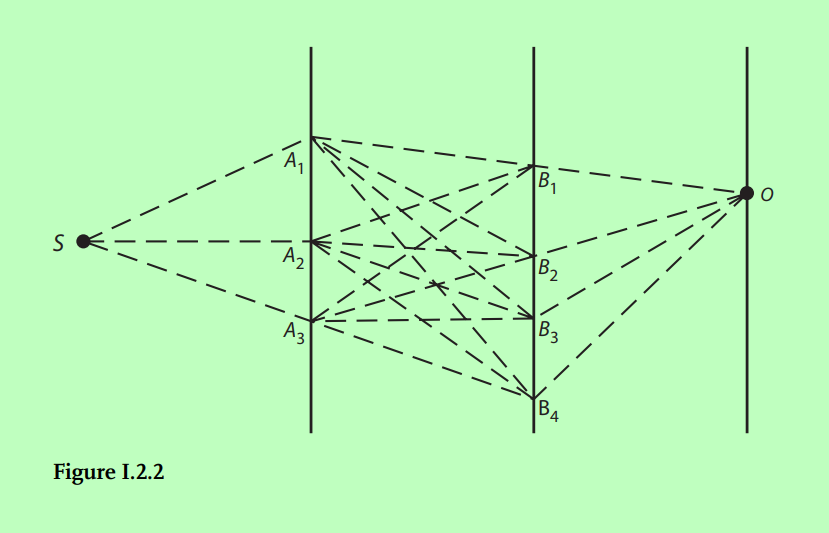
\includegraphics[scale=0.5]{picutres/multiple_slits.png} \\
%     \textit{Figure 1.2.2 from} \cite[Zee, QFT in a Nutshell]{ZeeQFTNutshell}
% \end{center}

% \vskip 0.5cm
% If we now imagine that the number of holes and the number of planes placed one after another both go to $\infty$ (i.e. we have empty space between $S$ and $O$), then it seems reasonable to say 

% \[ \mathcal{A}(S \rightarrow O) =  \sum_{\text{path } \gamma} \mathcal{A}\left(S \rightarrow O \text{ via } \gamma\right) \]

% and as we take the limits, this sum over paths made of straight segments approaches an integral over all smooth paths between $S$ and $O$. This is the general idea.


\vskip 0.5cm
\subsection{Path Integrals in Quantum Mechanics}



% %%%%%%%%%%%%%%%%%%%%%%%%%%%%%%%%%%%%%%%%%%%%%%
% \newpage
% \section{Fiber Bundles and Principal G-Bundles}
% %%%%%%%%%%%%%%%%%%%%%%%%%%%%%%%%%%%%%%%%%%%%%%
% \vskip 0.5cm


% %%%%%%%%%%%%%%%%%%%%%%%%%%%%%%%%%%%%%%%%%%%%%%
% \newpage
% \section{Connections on Bundles}
% %%%%%%%%%%%%%%%%%%%%%%%%%%%%%%%%%%%%%%%%%%%%%%
% \vskip 0.5cm


% %%%%%%%%%%%%%%%%%%%%%%%%%%%%%%%%%%%%%%%%%%%%%%
% \newpage
% \section{Connection 1-forms}
% %%%%%%%%%%%%%%%%%%%%%%%%%%%%%%%%%%%%%%%%%%%%%%
% \vskip 0.5cm


%%%%%%%%%%%%%%%%%%%%%%%%%%%%%%%%%%%%%%%%%%%%%%
\newpage
\section{Principal $G$-Bundles and Associated Bundles}
%%%%%%%%%%%%%%%%%%%%%%%%%%%%%%%%%%%%%%%%%%%%%%
% \vskip 0.5cm

\begin{bluebox}
    This section is heavily based off \cite{SchullerGeomAnatomy} and \cite{SkinnerAQFT}.
\end{bluebox}

\subsection{Some motivation}
Of great importance to our modern understanding of particle physics are \emph{Yang-Mills} type theories. These are examples of \textbf{Non-Abelian gauge theories}, and "the starting point for any non-Abelian gauge theory is the statement that our world is not just a manifold $M$, but rather a \emph{principal $G-$bundle}"\cite{SkinnerAQFT}. In this section we'll define these objects, but before that...

\subsection*{Let's recall some facts about Bundles}

Recall that the tangent bundle is the triple $(TM, \pi, M)$ where \[ TM = \coprod_{x \in M} T_x M \] A fiber of the map $\pi$ is a tangent space, and a section of $\pi$ is a vector field $X$. Similarly, a cotangent bundle is a triple $(T^*M, \pi, M)$ where \[ TM = \coprod_{x \in M} T_x^* M \] and, this time, a fiber is a cotangent space whereas a section is a one-form $\omega$.
\\
\\
Recall that if we have a map $f \text{ : } M \rightarrow N$ between smooth manifolds, this induces a \textbf{pushforward} for tangent vectors and a \textbf{pullback} for cotangent vectors.

\begin{center}
    \[ \begin{tikzcd}
	TM & TN && {T^*M} & {T^*N} \\
	M & N && M & N
	\arrow["{(f_*)}", from=1-1, to=1-2]
	\arrow["{(f^*)}"', from=1-5, to=1-4]
	\arrow["X", from=2-1, to=1-1]
	\arrow["f"', from=2-1, to=2-2]
	\arrow["{(f_*)(X)}"', from=2-2, to=1-2]
	\arrow["\omega", from=2-4, to=1-4]
	\arrow["f"', from=2-4, to=2-5]
	\arrow["{(f^*)(\omega)}"', from=2-5, to=1-5]
\end{tikzcd} \]
\end{center}

The pullback satisfies $(f^*\omega)(X) = \omega(f_* X)$ for $\omega \in \mathfrak{X}^{*}(N)$ and $X \in \mathfrak{X}(M)$.

\vskip 0.5cm
\subsection*{Also, let's recall some facts about Lie Groups and Lie Algebras}

Let $G$ be a Lie-Group and let $g, h \in G$. A \textbf{left $g$-translation} is described by 
\begin{align*}
    L_g \text{ : } &G \rightarrow G \\
    &h \mapsto g \cdot h
\end{align*} and similarly a \textbf{right $g-$translation} is described by 
\begin{align*}
    R_g \text{ : } &G \rightarrow G \\
    &h \mapsto  h \cdot g
\end{align*} Since $G$ is a Lie Group (and so, a smooth manifold), left and right actions are \textbf{diffeomorphisms} of $G$. As such, the pushforward $(L_g)_*$ is well-defined. 
\\
\\
A vector field $X$ on $G$ such that $(L_g)_*(X) = X$ for every $g \in G$ is said to be \textbf{left-invariant}, and the set of left-invariant vector fields forms the \textbf{Lie Algebra $\mathfrak{g}$ of the Lie Group $G$}. It is also denoted as $\mathcal{L}(G)$ or $\mathrm{Lie}(G)$.

\begin{bluebox}
    Recall that an \textbf{algebra} is a vector-space $V$ equipped with a bilinear product $[ \_, \_ ] \text{ : } V \times V \rightarrow V$. A lie-algebra is an algebra whose product satisfies the \textbf{Jacobi-Identity} i.e. \[ [v, [w , z]] + [z, [v, w]] + [w, [z, v]] = 0 \] for all $v, w, z \in V$.
    \\
    \\
    The set of left-invariant vector fields is a particularly important lie-algebra and so we give it the grand title "Lie algebra \textit{of} the Lie Group". The reason for this is in the next theorem.
\end{bluebox}

\vskip 0.5cm
\begin{redbox}
    \begin{theorem}
        For a lie group $G$, $\mathcal{L}(G) \cong T_e G$ i.e. the lie algebra is isomorphic to the tangent space at the identity. 
    \end{theorem}
\end{redbox}

\begin{proof}
    Fill in later.
\end{proof}

\vskip 0.5cm
\subsection{$G$-actions, Orbits, Orbit Space}

Left and Right Translations can be thought of as special cases of \textbf{lie group actions}.

\begin{definition}
    Given a Lie group $G$ and smooth manifold $M$, a \textbf{left $G$-action} is a smooth map 
    \begin{align*}
        \triangleright \text{ : } G \times M &\rightarrow M \\
        (g, p) &\mapsto g \triangleright p
    \end{align*} such that 
    \begin{enumerate}
        \item $e \triangleright p = p$, for any $p \in M$ and 
        \item $g_1 \triangleright \left( g_1 \triangleright p \right) = (g_1 \cdot g_2) \triangleright p$ for any $p \in M$ and $g_1, g_2 \in G$
    \end{enumerate}
\end{definition}

Right $G-$actions can be defined analogously. We call a manifold $M$ equipped with a left-$G$ action on it as a $G-$manifold. Now, given a point $p \in M$ we call the set of all possible points in $M$ that can be reached from $p$ via a $G-$action as the \textbf{Orbit of $p$} i.e.

\begin{definition}
    Given a smooth $G$-manifold $M$, the Orbit of $p$ is \[ G_p = \{ q \in M \;|\; q = g \triangleright p, \text{ for some } g \in G \} \]
\end{definition}

\textit{Example:} Consider $M = \mathbb{R}^2$ and consider the action of the matrix representation of $SO(2)$. The orbit of $p \in \mathbb{R}^2$ is the circle of radius $|p|$ centered around the origin.
\begin{center}
    \includegraphics*[scale=0.30]{pictures/Schuller_orbit_ofSO(2).png} \\
    \cite[Pg. 165]{SchullerGeomAnatomy}
\end{center}

If we introduce an equivalence relation $\sim$ such that $p, m \sim M$ are $p \sim q$ if and only if there exists some $g \in G$ so that $q = g \triangleright p$ then the equivalence classes are exactly the orbits. 

\begin{definition}
    For action $\triangleright \text{ : } G \times M \rightarrow M$ we define the \textbf{Orbit Space} to be 
    \[ M/G = \left(M/\sim\right) = \{ G_p \; | \; p \in M \} \]
    i.e. the collection of all orbits under the action.
\end{definition}

\begin{definition}
    Similarly, the \textbf{Stabilizer} of some $p \in M$ under the $G-$action is the set of $g \in G$ which leave it invariant i.e. \[ S_p = \{ g \in G\; | \; g \triangleright p = p \}  \]
\end{definition}

Two important classes of $G$-actions are:
\begin{itemize}
    \item \textbf{Free Actions:} those actions such that $S_p = \{e\}$ for all $p \in M$. These are unrestricted and chaotic (hence "free") in the sense that there is no redundancy of different $g \in G$ sending $p$ to itself.
    \item \textbf{Transitive Actions: } those actions such that for all $p, q \in M$ there must exist some $g \in G$ such that $q = g \triangleright p$. So, we can \emph{always} get from one point to another via the $G$-action.
\end{itemize}

Notably,
\begin{theorem}
    If $\triangleright \text{ : } G \times M \rightarrow M$ is a \textbf{free} action, then $G_p \cong G$ for all $p \in M$.
\end{theorem}
i.e. each orbit is isomorphic to the original Lie Group.
\\
\\
\begin{proof}
    (Sketch) Fix $p \in P$. The action is free meaning the only way to have $h \triangleright p = p$, $h \in G$ is for $h = e$. Then, $G_p$ is a group because it has a unique identity element $e \triangleright p = p$ and has group structure due to the definition of a left $G-$action.
    \\
    \\
    Then, the map $g \mapsto g \triangleright p$ is a group isomorphism.
\end{proof}
\\
\\
\begin{thought}
    {Give an example for why this is cool.}
\end{thought}
\\
\\
All of these results hold for \textbf{right-actions} as well, and the proofs follow the same reasoning, just with slight modifications.

\vskip 0.5cm
\subsection{Principal $G$-Bundles}

\begin{definition}
    Let $G$ be a lie group. A smooth bundle $(E, \pi, M)$ is called a \textbf{G-principal bundle} if $E$ is equipped with a \textbf{free, right (not left!) $G-$action} such that \[\begin{tikzcd}
	E & E \\
	M & {E/G}
	\arrow[""{name=0, anchor=center, inner sep=0}, "\pi"', from=1-1, to=2-1]
	\arrow[""{name=1, anchor=center, inner sep=0}, "\rho", from=1-2, to=2-2]
	\arrow["{\cong_{\text{iso}}}"{description}, draw=none, from=0, to=1]
\end{tikzcd}\] where $\rho$ is the quotient map sending $p \in E$ to its equivalence class in the orbit space $E/G$ \textbf{and} the right action \textbf{preserves the fiber} i.e. for any $p \in E$ and $g \in G$ we have $\pi(p) = \pi(p \triangleleft g)$
\end{definition}

\begin{bluebox}
    Note that each fiber of $(E, \rho, E/G)$ is an orbit and, because we have a \emph{free} action, is isomorphic to $G$.
\end{bluebox}

In physics, $G$ is often called the Gauge group, whereas in math it's called the Structure group.

\begin{redbox}
    \textbf{Why do we consider a right action instead of a left action?}
    \\
    \\
    Fill in later.
\end{redbox}

\subsection*{Transition Maps}



\begin{note}
    {Add more theorems eg. related to triviality}
\end{note}

\vskip 0.5cm
\subsection{Associated Principal Bundles}

%%%%%%%%%%%%%%%%%%%%%%%%%%%%%%%%%%%%%%%%%%%%%%
\newpage
\section{Connections on Bundles}
%%%%%%%%%%%%%%%%%%%%%%%%%%%%%%%%%%%%%%%%%%%%%%
\vskip 0.25cm

For any matter-field theory, if we wish to write down the Kinetic terms, we need to be able to find velocities i.e. we need to calculate derivatives. We might naiv$\ddot{e}$ly write the following expression for velocity \[ v^{\mu} \partial_{\mu} \phi(x) = \lim_{\epsilon \rightarrow 0} \frac{\phi(x + \epsilon v) - \phi(x)}{\epsilon} \] where $v$ is a vector at position $x$. But, for a charged field $\phi$, $\phi(x + \epsilon v)$ and $\phi(x)$ belong to \emph{different fibers}: $E_{x + \epsilon v}$ and $E_{x}$ respectively.
\\
\\
In order to compare quantities in different fibers, we need to add more structure. We define a \textbf{connection}, which allows us to conduct \textbf{parallel transport}, and in the special case where each fiber has vector space structure the connection further gives us a \textbf{covariant derivative}.
\\
\\
\subsection{Pictorial view: Vertical and Horizontal Subspaces, Connections}
A connection is essentially just a procedure to smooth move from one fiber to another which is infitessimally close to the first.
\begin{center}
    \includegraphics*[scale=0.15]{pictures/Infinitessimally_close_fibers.png}
\end{center}
Intuitively, we might think of moving from one fiber to the other by some vertical distance prescribed as a function of the point in $M$ corresponding to the fiber.
\\
\\ 
We'll make this more precise by defining the \textbf{vertical} and \textbf{horizontal} subspaces of the tangent space at each point of $P$, and use them to encode this prescription.
\\
\\
What makes a vector "vertical" or "horizontal"? Pictorially, we can consider a path through $P$ (the grey dotted lines) and consider a vector along the path. Then, the bundle's projection map $\pi$ allows us to project the path in $P$ down to a path in $M$. 
\\
\\
Visually, we see that a "vertical" vector remains along the fiber itself after projection whereas the horizontal one does not. 
\begin{note}
    {The proj of the vertical vector should just be a point. Edit the picture.}
\end{note} 
\begin{center}
    \includegraphics*[scale=0.15]{pictures/Hor-and-Ver-vectors.png}
\end{center}
This motivates the following definition:
\begin{definition}
    Let $(P, \pi, M)$ be a principal $G-$bundle with typical fiber $F$. For $p \in P$, we define the \textbf{Vertical Subspace} $V_{p} P$ of $T_{p} P$ to be \[ V_p P = \ker((\pi_*)_p) = \{ X \in T_p P \; | \; (\pi_*)_p (X) = 0 \} \]
\end{definition}

Now, we define a (NOT \emph{the}) Horizontal subspace as 
\begin{definition}
    Given the priincipal $G-$bundle $(P, \pi, M)$, a horizontal subspace at $p \in P$ is a vector subspace $H_p P$ of $T_p P$ such that \[ T_p P = V_p P \oplus H_p P \] 
\end{definition}

While the vertical subspace is fixed for a point $p \in P$ (it's the collection of \emph{all} the velocity vectors that lie along the Fiber), there isn't one unique $H_p P$ - instead there is a continuous spectrum of choices we can pick from.
\begin{center}
    \includegraphics*[scale=0.15]{pictures/VpP-and-HpP.png}
\end{center}
Consider the vector $\vec{v}$ above. If we choose $H_p P$ along the solid green line and decompose $\vec{v}$ into its components along $V_p P$ and $H_p P$, then it has non-zero vertical component. If instead we choose $H_pP$ to lie along the dashed green line, then the vertical component of $\vec{v}$ is zero! 
\\
\\
So, the vertical component is decided by the Horizontal Subspace we choose. If we consider two fibers that are infinitessimally close to each other, then we can describe the connection as being a vector in $H_p P$.
\\
\\
Though technically $H_p P$ is distinct from $H_{p'} P$ (where $p'$ is the point in $P$ infinitessimally close to $p$ under consideration), the error between simply "adding $\vec{v}$" versus using the exponential map to be go from the fiber to the manifold $P$ is negligible \emph{because} the points are infinitessimally close! 
\begin{thought}
    {Inspect this explanation.}
\end{thought}

\begin{bluebox}
    \textbf{Thus, a choice of Horizontal Subspace is equivalent to a choice of connection!}
\end{bluebox}

Later on, we'll describe how a connection allows us to \textbf{parallel transport} essentially by integrating all the small changes (each small change is described by the connection).

So, we make the following definition:
\begin{definition}
    A \textbf{connection} on a Principal $G-$bundle $P \xrightarrow{\pi} M$ is an assignment (really, a \emph{smooth distribution}) where for each $p \in P$, a vector subspace $H_p P$ of $T_p P$ is chosen so that 
    \begin{enumerate}[label=(\alph*)]
        \item $ T_p P = V_p P \oplus H_p P $ i.e. $H_p P$ is a horizontal subspace.
        \item $\left(\triangleleft g\right)_* (H_p P) = H_{p \triangleleft g} P$ 
        \item The unique decomposition for any $X_p \in T_p P$ as \[ X_p = hor(X_p) + ver(X_p) \] where, by definition, $hor(X_p) \in H_p P$ and $ver(X_p) \in V_p P$ leads, for every \underline{smooth} vector field $X \in \Gamma(TP)$, to two \underline{smooth} vector fields $hor(X)$ and $ver(X)$.
    \end{enumerate}
\end{definition}
The second condition is the requirement that if we move \emph{along the fiber} from $p$ to $p \triangleleft g$, then the Horizontal Subspace $H_{p \triangleleft g} P$ defined by the connection is equal the pushforward of $H_p P$ by $\triangleleft g$. 
\\
\\
The third condition essentially enforces that if we move along a smooth path in $P$ (not necessarily along any one fiber) then the choice of $H_p P$ is smooth.
\\
\\
Okay, cool. We've defined a connection and its conditions, but how do we actually describe this "choice of horizontal subspace"-function? It turns out we can encode all of the information into a single Lie-algebra valued $1-$form called the \textbf{Connection 1-form}.
\\
\\
We'll see that the Connection 1-form satsfies the certain list of properties, and in fact, \emph{every} 1-form on $P$ that satisfies these properties defines some connection. 

\subsection{Connection 1-forms}




\subsection{Curvature and Curvature 2-forms}

%%%%%%%%%%%%%%%%%%%%%%%%%%%%%%%%%%%%%%%%%%%%%%
\newpage
\section{TQFTs I}
%%%%%%%%%%%%%%%%%%%%%%%%%%%%%%%%%%%%%%%%%%%%%%
\vskip 0.5cm


%%%%%%%%%%%%%%%%%%%%%%%%%%%%%%%%%%%%%%%%%%%%%%
\newpage
\section{TQFTs II}
%%%%%%%%%%%%%%%%%%%%%%%%%%%%%%%%%%%%%%%%%%%%%%
\vskip 0.5cm


%%%%%%%%%%%%%%%%%%%%%%%%%%%%%%%%%%%%%%%%%%%%%%
\newpage
\section{BRST Quantization}
%%%%%%%%%%%%%%%%%%%%%%%%%%%%%%%%%%%%%%%%%%%%%%
\vskip 0.5cm
Explain stuff.


\vskip 0.5cm
\subsection{BRST Cohomology}

In a theory with gauge-symmetry, we have redundancy. 


%%%%%%%%%%%%%%%%%%%%%%%%%%%%%%%%%%%%%%%%%%%%%%
\newpage
% \section{References}
%%%%%%%%%%%%%%%%%%%%%%%%%%%%%%%%%%%%%%%%%%%%%%
\vskip 0.5cm
\bibliographystyle{plain} % We choose the "plain" reference style
\bibliography{refs} % Entries are in the refs.bib file


\end{document}